\documentclass[a4paper,12pt]{report}

\usepackage[utf8]{inputenc}
\usepackage[T1]{fontenc}
\usepackage{array}
\usepackage{amsmath}
\usepackage[english]{babel}
\usepackage{graphicx}
\usepackage[a4paper]{geometry}
\usepackage[colorlinks=true,urlcolor=blue,linkcolor=blue]{hyperref}
\usepackage{url}
\usepackage[nottoc,numbib]{tocbibind}
\usepackage{color}
\usepackage{epstopdf}
\usepackage{xcolor}
\usepackage[backend=biber,style=phys]{biblatex}

\addbibresource{../Bibliography.bib}

\makeatletter
	\renewcommand{\thechapter}{\Roman{chapter}}
\makeatother

\begin{document}

\chapter{Optical control of an individual Cr spin in a CdTe QD}
	
	Lorem ipsum dolor sit amet, consectetur adipiscing elit. Curabitur tortor quam, imperdiet quis facilisis sed, fringilla a quam. Cras ante odio, hendrerit ac ante nec, cursus imperdiet urna. Mauris convallis ultricies purus, nec condimentum erat bibendum vel. Aliquam erat volutpat. Pellentesque condimentum, eros a consequat accumsan, turpis sem euismod nisi, sed fringilla quam turpis sit amet erat. Mauris dictum odio sed nisi dapibus, et molestie mauris rutrum. Praesent convallis dolor in nibh blandit bibendum. Quisque sit amet arcu consectetur lorem luctus venenatis nec quis dui. Aliquam erat volutpat. Aenean auctor elit nec tristique dignissim. Nulla massa mi, efficitur semper ex id, pretium eleifend massa. Vivamus sit amet orci scelerisque, gravida est ut, vulputate odio.
	
	\section{Optical pumping and spin dynamics in a Cr doped QD}
	
		\subsection{Resonant optical pumping of the Cr spin}
		
		Lorem ipsum dolor sit amet, consectetur adipiscing elit. Curabitur tortor quam, imperdiet quis facilisis sed, fringilla a quam. Cras ante odio, hendrerit ac ante nec, cursus imperdiet urna. Mauris convallis ultricies purus, nec condimentum erat bibendum vel. Aliquam erat volutpat. Pellentesque condimentum, eros a consequat accumsan, turpis sem euismod nisi, sed fringilla quam turpis sit amet erat. Mauris dictum odio sed nisi dapibus, et molestie mauris rutrum. Praesent convallis dolor in nibh blandit bibendum. Quisque sit amet arcu consectetur lorem luctus venenatis nec quis dui. Aliquam erat volutpat. Aenean auctor elit nec tristique dignissim. Nulla massa mi, efficitur semper ex id, pretium eleifend massa. Vivamus sit amet orci scelerisque, gravida est ut, vulputate odio.
		
	\begin{figure}[h!]
	\begin{center}
		\includegraphics[width=14.9cm]{Pictures/PumpPres.png}
	\end{center}
	\caption{Low temperature PL spectra of QD2 exciton in co-polarized excitation and detection for B = 0T. Inset: Schematic of the energy levels in a Cr-doped QD and configuration of excitation/detection for resonant optical pumping. The ground states $S_z = 0$, $\pm1$ are split by the magnetic anisotropy $D_0 S_z^2$. In the excited state (X-Cr), the exchange interaction with the bright exciton ($|\pm1\rangle$) split the states $S_z = \pm1$. The higher energy Cr states, $S_z = \pm2$, are not displayed.}
	\label{PumpPres}
	\end{figure}
	
	Curabitur eget ipsum egestas dui viverra suscipit. Cras aliquet lacus vitae erat finibus semper. Nulla pharetra eget urna vitae sodales. Nunc faucibus velit lacus, nec ornare eros aliquet quis. Donec a orci nec sem pulvinar ultricies sit amet ut arcu. Nullam id vehicula enim, at tincidunt velit. Duis vestibulum lorem a molestie fringilla. Nullam tincidunt semper placerat. Donec nibh sem, ornare eget cursus ac, luctus sit amet eros. Phasellus eget interdum nisi. Donec mollis risus id lectus fringilla, et commodo risus iaculis. Donec at lacus sed nibh posuere posuere sit amet eget sapien. In dignissim, enim sit amet convallis fermentum, lacus nulla gravida tortor, non facilisis ex nisl sit amet augue. Maecenas eu enim condimentum, consectetur ligula vel, tincidunt nisl. Nam laoreet dictum volutpat. Donec at erat venenatis, ultrices lorem ac, vestibulum neque.
	
	\begin{figure}[h!]
	\begin{center}
		\includegraphics[width=10cm]{../FillingPicture.png}
	\end{center}
	\caption{Resonant optical pumping experimental setup}
	\label{PumpExpSetup}
	\end{figure}	
		
	Curabitur eget ipsum egestas dui viverra suscipit. Cras aliquet lacus vitae erat finibus semper. Nulla pharetra eget urna vitae sodales. Nunc faucibus velit lacus, nec ornare eros aliquet quis. Donec a orci nec sem pulvinar ultricies sit amet ut arcu. Nullam id vehicula enim, at tincidunt velit. Duis vestibulum lorem a molestie fringilla. Nullam tincidunt semper placerat. Donec nibh sem, ornare eget cursus ac, luctus sit amet eros. Phasellus eget interdum nisi. Donec mollis risus id lectus fringilla, et commodo risus iaculis. Donec at lacus sed nibh posuere posuere sit amet eget sapien. In dignissim, enim sit amet convallis fermentum, lacus nulla gravida tortor, non facilisis ex nisl sit amet augue. Maecenas eu enim condimentum, consectetur ligula vel, tincidunt nisl. Nam laoreet dictum volutpat. Donec at erat venenatis, ultrices lorem ac, vestibulum neque.
	
	\begin{figure}[h!]
	\begin{center}
		\includegraphics[width=14.9cm]{Pictures/PumpResults.eps}
	\end{center}
	\caption{(a) PL transients recorded in circular polarization on line (3) and on line (4) (as defined in the inset) under the resonant (pump on (1)) and quasi-resonant (probe at $E_{exc.}\approx 2068$ meV) optical excitation sequences displayed at the bottom. Inset: PL of X-Cr and configuration of the resonant excitation and detection. (c) and (d): Energy detuning dependence of resonant PL intensity ($I_1$, at the beginning and $I_2$, at the end of the pump pulse) and of the corresponding normalized amplitude of pumping transient ($I_1-I_2)/I_2$.}
	\label{PumpingExp}
	\end{figure}		
		
	Curabitur eget ipsum egestas dui viverra suscipit. Cras aliquet lacus vitae erat finibus semper. Nulla pharetra eget urna vitae sodales. Nunc faucibus velit lacus, nec ornare eros aliquet quis. Donec a orci nec sem pulvinar ultricies sit amet ut arcu. Nullam id vehicula enim, at tincidunt velit. Duis vestibulum lorem a molestie fringilla. Nullam tincidunt semper placerat. Donec nibh sem, ornare eget cursus ac, luctus sit amet eros. Phasellus eget interdum nisi. Donec mollis risus id lectus fringilla, et commodo risus iaculis. Donec at lacus sed nibh posuere posuere sit amet eget sapien. In dignissim, enim sit amet convallis fermentum, lacus nulla gravida tortor, non facilisis ex nisl sit amet augue. Maecenas eu enim condimentum, consectetur ligula vel, tincidunt nisl. Nam laoreet dictum volutpat. Donec at erat venenatis, ultrices lorem ac, vestibulum neque.

	\begin{figure}[h!]
	\begin{center}
		\includegraphics[width=15cm]{Pictures/ContProbe.eps}
	\end{center}
	\caption{PL transient recorded when probing with a laser tuned in resonance with (a) the line (1) and detecting on the line (4), and (b) the line (4) and detecting on the line (1). Unlike in Fig.~\ref{PumpingExp} where the quasi-resonant laser was only turned on for a short amount of time, it was now left on during the entirety of the measurement.}
	\label{ContProbe}
	\end{figure}

	Curabitur eget ipsum egestas dui viverra suscipit. Cras aliquet lacus vitae erat finibus semper. Nulla pharetra eget urna vitae sodales. Nunc faucibus velit lacus, nec ornare eros aliquet quis. Donec a orci nec sem pulvinar ultricies sit amet ut arcu. Nullam id vehicula enim, at tincidunt velit. Duis vestibulum lorem a molestie fringilla. Nullam tincidunt semper placerat. Donec nibh sem, ornare eget cursus ac, luctus sit amet eros. Phasellus eget interdum nisi. Donec mollis risus id lectus fringilla, et commodo risus iaculis. Donec at lacus sed nibh posuere posuere sit amet eget sapien. In dignissim, enim sit amet convallis fermentum, lacus nulla gravida tortor, non facilisis ex nisl sit amet augue. Maecenas eu enim condimentum, consectetur ligula vel, tincidunt nisl. Nam laoreet dictum volutpat. Donec at erat venenatis, ultrices lorem ac, vestibulum neque.
	
	\begin{figure}[h!]
	\begin{center}
		\includegraphics[width=14.9cm]{Pictures/PWProbe.eps}
	\end{center}
	\caption{PL transients measured under variation of the probe power: (a) $P_{probe} = $ $\mu$W. (b) $P_{probe} = $ $\mu$W. (c) $P_{probe} = $ $\mu$W. The pump was either off (dark line) or tuned in resonance with the (..) line at $P_{pump} = $ $\mu$W. [TODO: Add power values and line number.]}
	\label{PWProbe}
	\end{figure}	
		
	Curabitur eget ipsum egestas dui viverra suscipit. Cras aliquet lacus vitae erat finibus semper. Nulla pharetra eget urna vitae sodales. Nunc faucibus velit lacus, nec ornare eros aliquet quis. Donec a orci nec sem pulvinar ultricies sit amet ut arcu. Nullam id vehicula enim, at tincidunt velit. Duis vestibulum lorem a molestie fringilla. Nullam tincidunt semper placerat. Donec nibh sem, ornare eget cursus ac, luctus sit amet eros. Phasellus eget interdum nisi. Donec mollis risus id lectus fringilla, et commodo risus iaculis. Donec at lacus sed nibh posuere posuere sit amet eget sapien. In dignissim, enim sit amet convallis fermentum, lacus nulla gravida tortor, non facilisis ex nisl sit amet augue. Maecenas eu enim condimentum, consectetur ligula vel, tincidunt nisl. Nam laoreet dictum volutpat. Donec at erat venenatis, ultrices lorem ac, vestibulum neque.
	
	\begin{figure}[h!]
	\begin{center}
		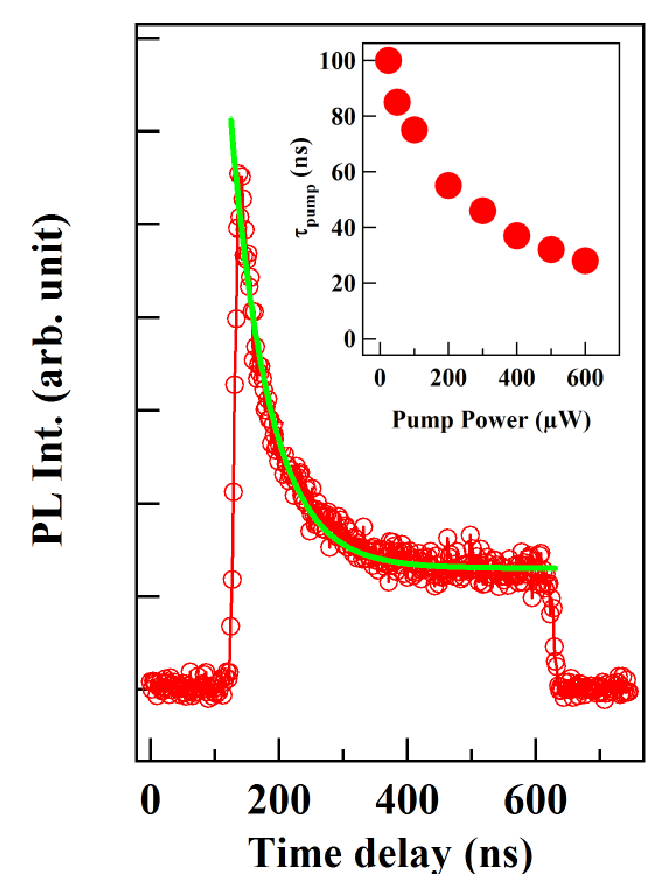
\includegraphics[width=7cm]{Pictures/PWPump.eps}
	\end{center}
	\caption{PL transient measured with the resonant pump pulse for a power $P_{probe} = $ $\mu$W. The exponential fit is drawn as a green line and gives a characteristic time of $\tau_{pump} = 60$ ns. The inset presents the evolution of $\tau_{pump}$ in function of the pumping laser power. [TODO: Reduce inset, add the $\tau_{pump}$ value.]}
	\label{PWPump}
	\end{figure}	
		
	Curabitur eget ipsum egestas dui viverra suscipit. Cras aliquet lacus vitae erat finibus semper. Nulla pharetra eget urna vitae sodales. Nunc faucibus velit lacus, nec ornare eros aliquet quis. Donec a orci nec sem pulvinar ultricies sit amet ut arcu. Nullam id vehicula enim, at tincidunt velit. Duis vestibulum lorem a molestie fringilla. Nullam tincidunt semper placerat. Donec nibh sem, ornare eget cursus ac, luctus sit amet eros. Phasellus eget interdum nisi. Donec mollis risus id lectus fringilla, et commodo risus iaculis. Donec at lacus sed nibh posuere posuere sit amet eget sapien. In dignissim, enim sit amet convallis fermentum, lacus nulla gravida tortor, non facilisis ex nisl sit amet augue. Maecenas eu enim condimentum, consectetur ligula vel, tincidunt nisl. Nam laoreet dictum volutpat. Donec at erat venenatis, ultrices lorem ac, vestibulum neque.	
	
	\begin{figure}[h!]
	\begin{center}
		\includegraphics[width=6cm]{Pictures/FillingPicture.png}
	\end{center}
	\caption{Heating in gap and far away from the dot}
	\label{Heating}
	\end{figure}
	
	Curabitur eget ipsum egestas dui viverra suscipit. Cras aliquet lacus vitae erat finibus semper. Nulla pharetra eget urna vitae sodales. Nunc faucibus velit lacus, nec ornare eros aliquet quis. Donec a orci nec sem pulvinar ultricies sit amet ut arcu. Nullam id vehicula enim, at tincidunt velit. Duis vestibulum lorem a molestie fringilla. Nullam tincidunt semper placerat. Donec nibh sem, ornare eget cursus ac, luctus sit amet eros. Phasellus eget interdum nisi. Donec mollis risus id lectus fringilla, et commodo risus iaculis. Donec at lacus sed nibh posuere posuere sit amet eget sapien. In dignissim, enim sit amet convallis fermentum, lacus nulla gravida tortor, non facilisis ex nisl sit amet augue. Maecenas eu enim condimentum, consectetur ligula vel, tincidunt nisl. Nam laoreet dictum volutpat. Donec at erat venenatis, ultrices lorem ac, vestibulum neque.
	
		
		\subsection{Dynamics of the Cr spin under optical excitation}
		
%			\subsubsection*{Autocorrelation and cross-correlation}		
		
		Lorem ipsum dolor sit amet, consectetur adipiscing elit. Curabitur tortor quam, imperdiet quis facilisis sed, fringilla a quam. Cras ante odio, hendrerit ac ante nec, cursus imperdiet urna. Mauris convallis ultricies purus, nec condimentum erat bibendum vel. Aliquam erat volutpat. Pellentesque condimentum, eros a consequat accumsan, turpis sem euismod nisi, sed fringilla quam turpis sit amet erat. Mauris dictum odio sed nisi dapibus, et molestie mauris rutrum. Praesent convallis dolor in nibh blandit bibendum. Quisque sit amet arcu consectetur lorem luctus venenatis nec quis dui. Aliquam erat volutpat. Aenean auctor elit nec tristique dignissim. Nulla massa mi, efficitur semper ex id, pretium eleifend massa. Vivamus sit amet orci scelerisque, gravida est ut, vulputate odio.
	
	\begin{figure}[h!]
	\begin{center}
		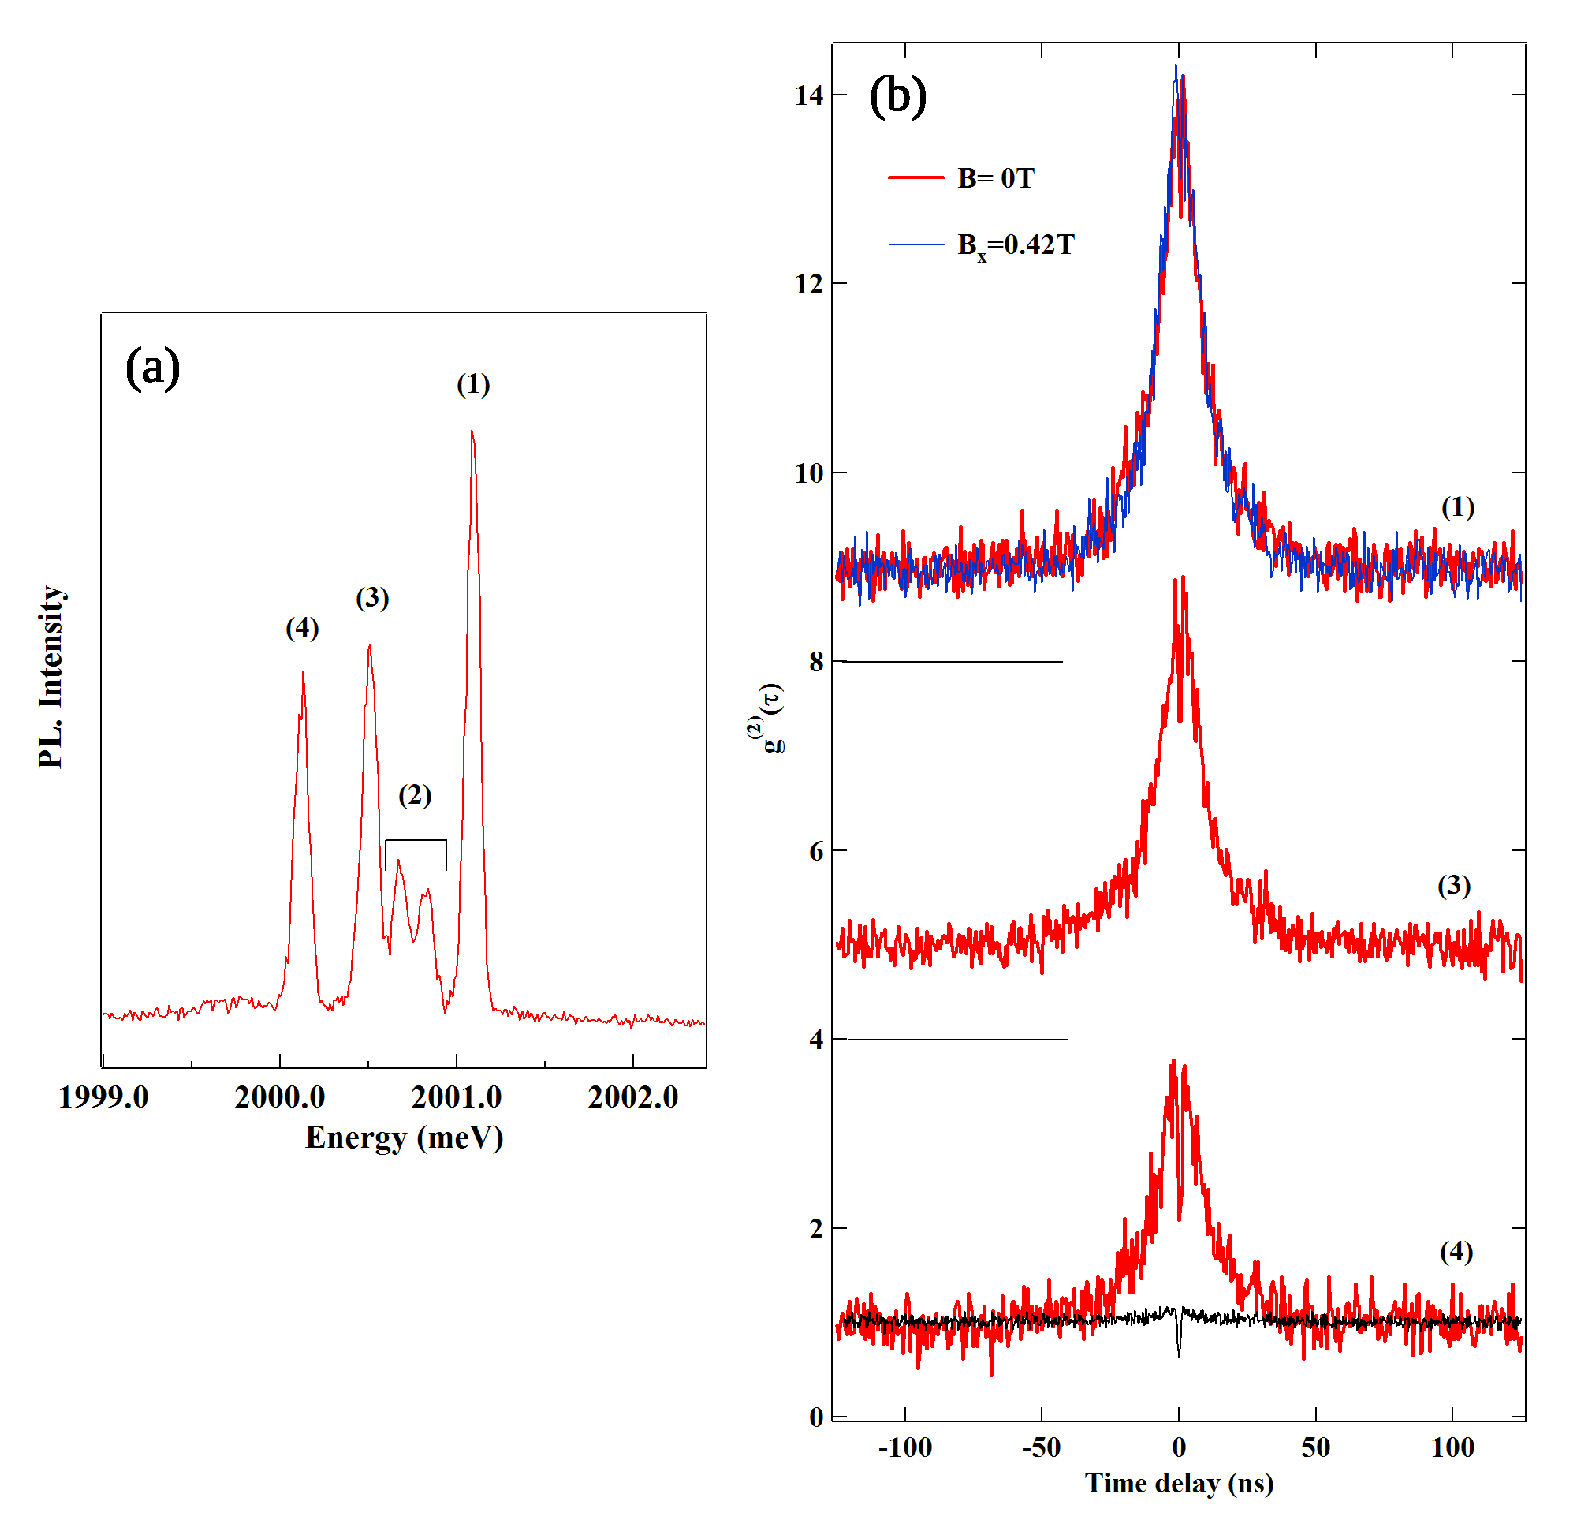
\includegraphics[width=7cm]{Pictures/AutocorPeaks.eps}
	\end{center}
	\caption{Auto-correlation of the PL intensity collected in circular polarization on the X-Cr lines (1), (4) and (5) (as defined in Fig.~\ref{PumpingExp}) and compared with the auto-correlation of the exciton in a non-magnetic QD (black line). The curves are shifted for clarity. For line (1), the auto-correlation is also recorded under a transverse magnetic field (blue line).}
	\label{AutocorPres}
	\end{figure}	
	
			To observe the time fluctuations of the Cr spin under CW optical excitation, we used the statistics of time arrivals of the photons emitted by a Cr-doped QD given by the second order correlation function g$^{(2)}(\tau)$ of the PL intensity. Fig.~\ref{AutocorExpCr} shows g$^{(2)}(\tau)$ for the lines (1), (3) and (4) recorded in circular polarization. These signals are compared with the auto-correlation obtained for the PL of a non-magnetic QD which is characteristic of a single-photon emitter with a dip (anti-bunching) at short delays. The width of the anti-bunching is given by the lifetime of the emitter and the generation rate of excitons and its depth is limited by the time resolution of the HBT setup. As illustrated in Fig.~\ref{AutocorExpCr}, typical non-magnetic CdTe/ZnTe QDs do not present any significant bunching induced by charge fluctuations \cite{QDAutocor,IndistPhoton}. A similar auto-correlation on a X-Cr PL line still presents a reduced coincidence rate near zero delay, but it is mainly characterized by a large photon bunching with a full width at half maximum (FWHM) in the 20 ns range. This large bunching reflects an intermittency in the emission of a given line of the QD coming from fluctuations of the Cr spin in a 10 ns timescale as it will be confirmed by cross-correlation measurements.

		The amplitude of the bunching reaches 5 for line (1) and is slightly weaker for the lower energy lines. In a simple picture of blinking where the selected QD line can be either in a state ON or OFF, the amplitude of the bunching is given by $\Gamma_{OFF}/\Gamma_{ON}$, ratio of the transition rates from OFF to ON, $\Gamma_{ON}$, and from ON to OFF, $\Gamma_{OFF}$ \cite{SubnanoSpectDiff}. An amplitude of bunching larger than 1 is then expected in a multilevel spin system where, after a spin relaxation, multiple spin-flips are usually required to come back to the initial state ($\Gamma_{ON}<\Gamma_{OFF}$). Let us finally note that the bunching signal is not affected by a weak transverse magnetic field ($B_x=0.42$T in Fig.~\ref{AutocorBandPW}). This confirms the presence of a large strain induced magnetic anisotropy $D_0$ which splits the Cr and X-Cr states and blocks their precession in a magnetic field.
		
	\begin{figure}[h!]
	\begin{center}
		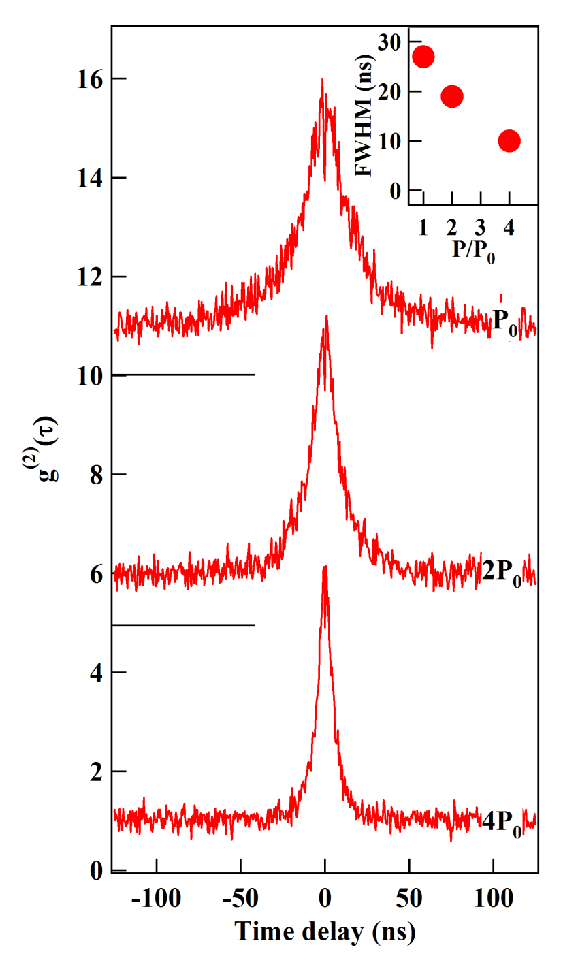
\includegraphics[width=7cm]{Pictures/AutocorPw.eps}
	\end{center}
	\caption{Auto-correlation of the PL intensity recorded in circular polarization on the high energy X-Cr line (1) for different excitation powers. The inset shows the corresponding FWHM of the bunching signal versus excitation power.}
	\label{AutocorPW}
	\end{figure}
	
	Curabitur eget ipsum egestas dui viverra suscipit. Cras aliquet lacus vitae erat finibus semper. Nulla pharetra eget urna vitae sodales. Nunc faucibus velit lacus, nec ornare eros aliquet quis. Donec a orci nec sem pulvinar ultricies sit amet ut arcu. Nullam id vehicula enim, at tincidunt velit. Duis vestibulum lorem a molestie fringilla. Nullam tincidunt semper placerat. Donec nibh sem, ornare eget cursus ac, luctus sit amet eros. Phasellus eget interdum nisi. Donec mollis risus id lectus fringilla, et commodo risus iaculis. Donec at lacus sed nibh posuere posuere sit amet eget sapien. In dignissim, enim sit amet convallis fermentum, lacus nulla gravida tortor, non facilisis ex nisl sit amet augue. Maecenas eu enim condimentum, consectetur ligula vel, tincidunt nisl. Nam laoreet dictum volutpat. Donec at erat venenatis, ultrices lorem ac, vestibulum neque.
	
	\begin{figure}[h!]
	\begin{center}
		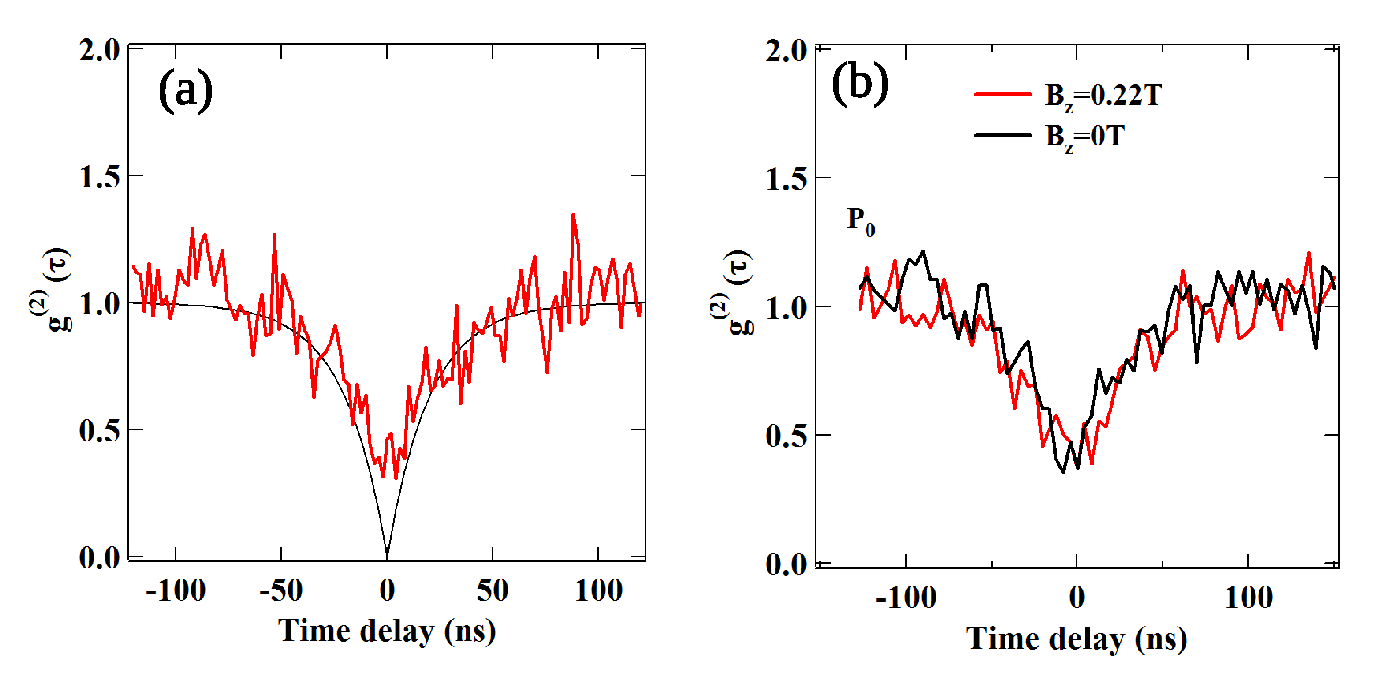
\includegraphics[width=12cm]{Pictures/CrosscorFit+B.eps}
	\end{center}
	\caption{(a) Correlation signal of the PL intensity of lines (1) and (4) recorded in the same circular polarization (cross-correlation) for three different excitation powers. The curves are shifted for clarity. The black line is an exponential fit with a characteristic time $\tau=20$ ns. (b) Longitudinal magnetic field dependence of the cross-correlation signal obtained at low excitation power.}
	\label{Crosscor}
	\end{figure}
	
	Curabitur eget ipsum egestas dui viverra suscipit. Cras aliquet lacus vitae erat finibus semper. Nulla pharetra eget urna vitae sodales. Nunc faucibus velit lacus, nec ornare eros aliquet quis. Donec a orci nec sem pulvinar ultricies sit amet ut arcu. Nullam id vehicula enim, at tincidunt velit. Duis vestibulum lorem a molestie fringilla. Nullam tincidunt semper placerat. Donec nibh sem, ornare eget cursus ac, luctus sit amet eros. Phasellus eget interdum nisi. Donec mollis risus id lectus fringilla, et commodo risus iaculis. Donec at lacus sed nibh posuere posuere sit amet eget sapien. In dignissim, enim sit amet convallis fermentum, lacus nulla gravida tortor, non facilisis ex nisl sit amet augue. Maecenas eu enim condimentum, consectetur ligula vel, tincidunt nisl. Nam laoreet dictum volutpat. Donec at erat venenatis, ultrices lorem ac, vestibulum neque.
	
%			\subsubsection{Relaxations through dark states}
%			
%		Lorem ipsum dolor sit amet, consectetur adipiscing elit. Curabitur tortor quam, imperdiet quis facilisis sed, fringilla a quam. Cras ante odio, hendrerit ac ante nec, cursus imperdiet urna. Mauris convallis ultricies purus, nec condimentum erat bibendum vel. Aliquam erat volutpat. Pellentesque condimentum, eros a consequat accumsan, turpis sem euismod nisi, sed fringilla quam turpis sit amet erat. Mauris dictum odio sed nisi dapibus, et molestie mauris rutrum. Praesent convallis dolor in nibh blandit bibendum. Quisque sit amet arcu consectetur lorem luctus venenatis nec quis dui. Aliquam erat volutpat. Aenean auctor elit nec tristique dignissim. Nulla massa mi, efficitur semper ex id, pretium eleifend massa. Vivamus sit amet orci scelerisque, gravida est ut, vulputate odio.
%	
%	\begin{figure}[h!]
%	\begin{center}
%		\includegraphics[width=10cm]{Pictures/FillingPicture.png}
%	\end{center}
%	\caption{Excitation power variations of the spectra and plot of the intensity of each peak}
%	\label{CrSpectraPwExp}
%	\end{figure}
%	
%	In order to study the different relaxation path of the system, probing of the emission evolution under excitation power was realized, reported on Fig.~\ref{CrSpectraPwExp}. As expected, the PL is becoming more intense with the augmentation of the excitation laser, since more exciton are produced and thus injected in the quantum dot. However, this power augmentation response is not the same for each of the peaks. The two central peaks, associated with the $|0\rangle$ states, start at about twice the intensity of the $|\pm1\rangle$ peaks for the most intense one, seemingly never reaching their maximum under our power range. However, when lowering the excitation power, they diminish quickly, and even seems to disappear at low energy, when exterior peaks still show luminescence. Plotting this evolution shows that the two central peaks exhibit a super-linear evolution. On the other side, the exterior peaks begin by rising in intensity before diminishing in a sub-linear fashion. This is coherent with the usual picture, where high power populating preferentially X$^2$-Cr states, while low power populates preferentially X-Cr states~\cite{??}. Finally, one can notice that the dark exciton exhibit the same behaviour, but the maximum emission intensity is at slightly lower power than the $|\pm1\rangle$.
%
%	\begin{figure}[h!]
%	\begin{center}
%		\includegraphics[width=10cm]{Pictures/FillingPicture.png}
%	\end{center}
%	\caption{Power variation simulation}
%	\label{CrSpectraPwMod}
%	\end{figure}
%	
%	The results of this evolution are well reproduced by our spin effective Hamiltonian, using the parameters found for the dot from the magneto-optics and the linear polarization fitting. The model results are presented in Fig.~\ref{CrSpectraPwMod}. [NOT SURE, TO BE REDISCUSSED]The super-linear behaviour of the central peaks can be explained by the proximity of dark exciton states. High power excitation can unlock radiative recombination path to states remaining non-radiative at low excitation power~\cite{PwSuperLinInc}. Such states linked to the $|0\rangle$ state make the emission on its peaks present a super-linear behaviour when excited at high power.
%
%		\subsection{Model of the spin dynamics}	
%
%	\begin{figure}[h!]
%	\begin{center}
%		\includegraphics[width=10cm]{Pictures/FillingPicture.png}
%	\end{center}
%	\caption{Simulation of autocorrelation on each peak and cross-correlation $|+1\rangle$ to $|+1\rangle$}
%	\label{SimulCRossAuto}
%	\end{figure}			
%		
%	To identify the main contribution to the observed spin fluctuations, we modelled the auto-correlation of the PL of X-Cr using the full spin level structure of a Cr-doped QD. We calculated the time evolution of the population of the twenty X-Cr states in the excited state of the QD and five Cr states in the ground state by solving numerically the master equation for the corresponding 25 x 25 density matrix $\rho$. The time evolution of the density matrix including relaxation and dephasing processes in the Lindblad form is given by $\partial \rho/\partial t=-i/\hbar[{\cal H},\rho]+L\rho$ where ${\cal H}$ is the Hamiltonian of the complete system ($X$-Cr and Cr) and $L\rho$ describes the coupling or decay channels resulting from an interaction with the environment \cite{SpinQJumps,ephBroad}. The energy levels of the Cr are controlled by the magnetic anisotropy $D_0S_z^2$. The X-Cr Hamiltonian, presented in Ref.\cite{LafuenteCrQD}, contains the energy of the Cr spin states, the carriers-Cr exchange interactions, the electron-hole exchange interaction in a confining potential of low symmetry and the structure of the valence band including heavy-hole/light-hole mixing. $D_0$ in the Cr Hamiltonian and the parameters in the X-Cr Hamiltonian cannot be precisely extracted from the zero magnetic field PL (Fig.~\ref{DotSpectra}(a)). For a qualitative description of the observed spin dynamics, we use in the model typical Cr-doped QD parameters extracted from magneto-optics measurements presented in Ref. \cite{LafuenteCrQD}. These parameters give a X-Cr splitting and a dark/bright excitons mixing similar to the one observed in the QD discussed in this article.
	
		\subsection{Spin relaxation in the dark}

		Lorem ipsum dolor sit amet, consectetur adipiscing elit. Curabitur tortor quam, imperdiet quis facilisis sed, fringilla a quam. Cras ante odio, hendrerit ac ante nec, cursus imperdiet urna. Mauris convallis ultricies purus, nec condimentum erat bibendum vel. Aliquam erat volutpat. Pellentesque condimentum, eros a consequat accumsan, turpis sem euismod nisi, sed fringilla quam turpis sit amet erat. Mauris dictum odio sed nisi dapibus, et molestie mauris rutrum. Praesent convallis dolor in nibh blandit bibendum. Quisque sit amet arcu consectetur lorem luctus venenatis nec quis dui. Aliquam erat volutpat. Aenean auctor elit nec tristique dignissim. Nulla massa mi, efficitur semper ex id, pretium eleifend massa. Vivamus sit amet orci scelerisque, gravida est ut, vulputate odio.
		
	\begin{figure}[h!]
	\begin{center}
		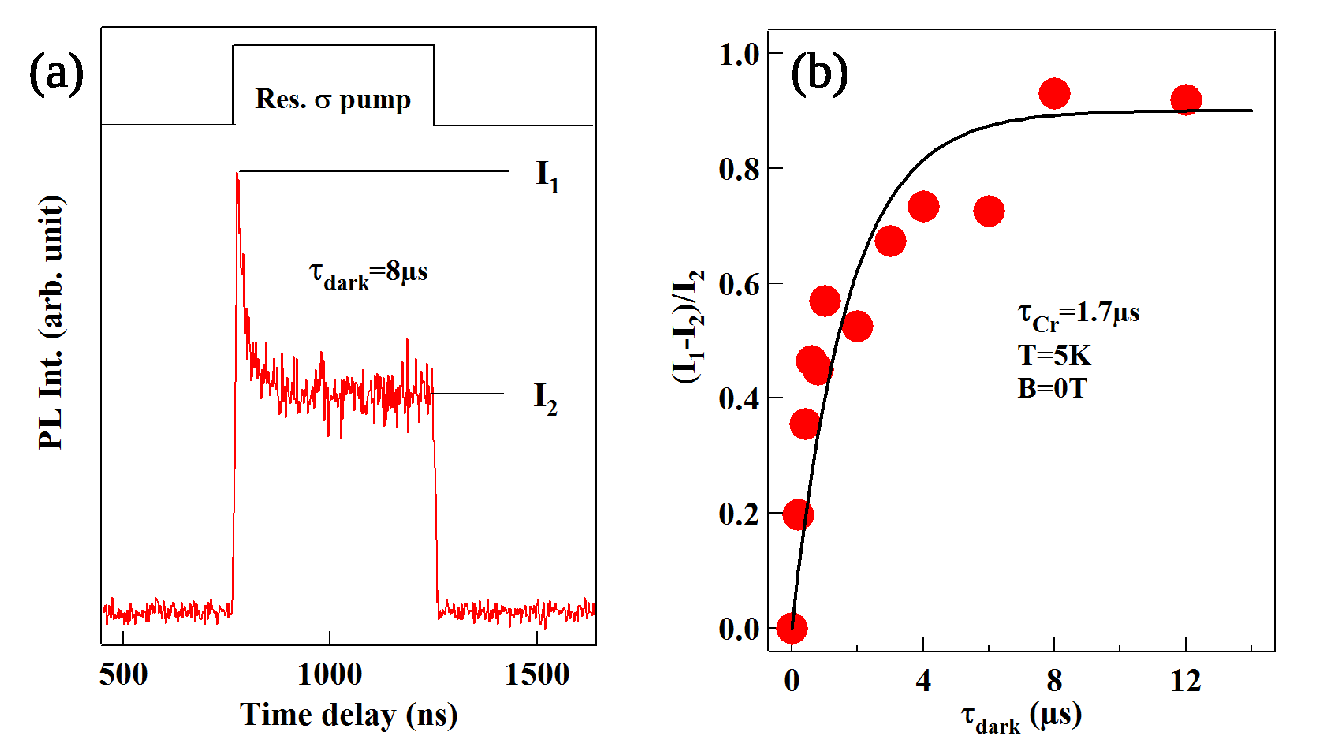
\includegraphics[width=12cm]{Pictures/RelaxDark.eps}
	\end{center}
	\caption{(a) Time evolution of the PL intensity of line (4) of X-Cr under resonant excitation on line (1) with a circularly polarized excitation pulse. (b) Evolution of the amplitude of the pumping transient $(I_1-I_2)/I_2$ as a function of the dark time between the excitation pulses. The black line is an exponential evolution with a characteristic time $\tau_{Cr}=1.7$ $\mu$s}
	\label{RelaxDark}
	\end{figure}		
		
	Curabitur eget ipsum egestas dui viverra suscipit. Cras aliquet lacus vitae erat finibus semper. Nulla pharetra eget urna vitae sodales. Nunc faucibus velit lacus, nec ornare eros aliquet quis. Donec a orci nec sem pulvinar ultricies sit amet ut arcu. Nullam id vehicula enim, at tincidunt velit. Duis vestibulum lorem a molestie fringilla. Nullam tincidunt semper placerat. Donec nibh sem, ornare eget cursus ac, luctus sit amet eros. Phasellus eget interdum nisi. Donec mollis risus id lectus fringilla, et commodo risus iaculis. Donec at lacus sed nibh posuere posuere sit amet eget sapien. In dignissim, enim sit amet convallis fermentum, lacus nulla gravida tortor, non facilisis ex nisl sit amet augue. Maecenas eu enim condimentum, consectetur ligula vel, tincidunt nisl. Nam laoreet dictum volutpat. Donec at erat venenatis, ultrices lorem ac, vestibulum neque.

	\begin{figure}[h!]
	\begin{center}
		\includegraphics[width=14.9cm]{Pictures/RelaxHeat.png}
	\end{center}
	\caption{Comparison of the relaxation of the Cr spin either after the quasi-resonant pulse (red, $E_{pump} = $ meV) or a resonant pump on the (..) line (blue). (a) Configuration to probe the relaxation after the quasi-resonant pulse. The dark time $\tau_{dark}$ between the quasi-resonant probe and the resonant pump is varied and the $\Delta I/I$ as defined in Fig.~\ref{PumpingExp} is calculated for each $\tau_{dark}$. (b) $\Delta I/I$ in function of the dark time $\tau_{dark}$ measured for the relaxation after a quasi-resonant pulse (red) or after a pumping pulse (blue). (c) Configuration to probe the relaxation after a resonant pulse, as presented in Fig.~\ref{RelaxDark}. [TODO: Replace "Time delay" in (b) with "Dark time". Add "Dark time on the configuration part. Add the wavelength of the probe and the line of the pump.]}
	\label{RelaxHeat}
	\end{figure}

	The $\Delta I/I$ evolution over dark time is used as a measure of the relaxation of the Cr spin: after a long enough time, both lines should stabilize at the same value.	

	\section{Optical Stark effect on an individual Cr spin}
		
		Lorem ipsum dolor sit amet, consectetur adipiscing elit. Curabitur tortor quam, imperdiet quis facilisis sed, fringilla a quam. Cras ante odio, hendrerit ac ante nec, cursus imperdiet urna. Mauris convallis ultricies purus, nec condimentum erat bibendum vel. Aliquam erat volutpat. Pellentesque condimentum, eros a consequat accumsan, turpis sem euismod nisi, sed fringilla quam turpis sit amet erat. Mauris dictum odio sed nisi dapibus, et molestie mauris rutrum. Praesent convallis dolor in nibh blandit bibendum. Quisque sit amet arcu consectetur lorem luctus venenatis nec quis dui. Aliquam erat volutpat. Aenean auctor elit nec tristique dignissim. Nulla massa mi, efficitur semper ex id, pretium eleifend massa. Vivamus sit amet orci scelerisque, gravida est ut, vulputate odio.	
	
	\begin{figure}[h!]
	\begin{center}
		\includegraphics[width=12cm]{Pictures/AutlerTownes.png}
	\end{center}
	\caption{Stark experiment}
	\label{StarkPres}
	\end{figure}	
	
		Lorem ipsum dolor sit amet, consectetur adipiscing elit. Curabitur tortor quam, imperdiet quis facilisis sed, fringilla a quam. Cras ante odio, hendrerit ac ante nec, cursus imperdiet urna. Mauris convallis ultricies purus, nec condimentum erat bibendum vel. Aliquam erat volutpat. Pellentesque condimentum, eros a consequat accumsan, turpis sem euismod nisi, sed fringilla quam turpis sit amet erat. Mauris dictum odio sed nisi dapibus, et molestie mauris rutrum. Praesent convallis dolor in nibh blandit bibendum. Quisque sit amet arcu consectetur lorem luctus venenatis nec quis dui. Aliquam erat volutpat. Aenean auctor elit nec tristique dignissim. Nulla massa mi, efficitur semper ex id, pretium eleifend massa. Vivamus sit amet orci scelerisque, gravida est ut, vulputate odio.
		
	\begin{figure}[h!]
	\begin{center}
		\includegraphics[width=14.9cm]{Pictures/StarkSplitDet.png}
	\end{center}
	\caption{(a) PL of X-Cr and configuration of excitation in the resonant optical control experiments. The inset illustrate the laser induced splittings in the ground and excited states for a $\sigma+$ excitation on $S_z=-1$. (b) PL intensity maps of lines (5) and (4) for an excitation on (1) as a function of the detuning (top) and of the excitation intensity (bottom). The PL is produced by a second non-resonant laser.}
	\label{StarkSplitandDet}
	\end{figure}		

	Curabitur eget ipsum egestas dui viverra suscipit. Cras aliquet lacus vitae erat finibus semper. Nulla pharetra eget urna vitae sodales. Nunc faucibus velit lacus, nec ornare eros aliquet quis. Donec a orci nec sem pulvinar ultricies sit amet ut arcu. Nullam id vehicula enim, at tincidunt velit. Duis vestibulum lorem a molestie fringilla. Nullam tincidunt semper placerat. Donec nibh sem, ornare eget cursus ac, luctus sit amet eros. Phasellus eget interdum nisi. Donec mollis risus id lectus fringilla, et commodo risus iaculis. Donec at lacus sed nibh posuere posuere sit amet eget sapien. In dignissim, enim sit amet convallis fermentum, lacus nulla gravida tortor, non facilisis ex nisl sit amet augue. Maecenas eu enim condimentum, consectetur ligula vel, tincidunt nisl. Nam laoreet dictum volutpat. Donec at erat venenatis, ultrices lorem ac, vestibulum neque.
	
	\begin{figure}[h!]
	\begin{center}
		\includegraphics[width=7cm]{Pictures/StarkDark.eps}
	\end{center}
	\caption{PL of line (1) and (2) (high energy line) for a laser on resonance with the dark exciton state (5). Inset: PL intensity map of line (1) as a function of the laser detuning around (5).}
	\label{DarkExcSplit}
	\end{figure}

	Curabitur eget ipsum egestas dui viverra suscipit. Cras aliquet lacus vitae erat finibus semper. Nulla pharetra eget urna vitae sodales. Nunc faucibus velit lacus, nec ornare eros aliquet quis. Donec a orci nec sem pulvinar ultricies sit amet ut arcu. Nullam id vehicula enim, at tincidunt velit. Duis vestibulum lorem a molestie fringilla. Nullam tincidunt semper placerat. Donec nibh sem, ornare eget cursus ac, luctus sit amet eros. Phasellus eget interdum nisi. Donec mollis risus id lectus fringilla, et commodo risus iaculis. Donec at lacus sed nibh posuere posuere sit amet eget sapien. In dignissim, enim sit amet convallis fermentum, lacus nulla gravida tortor, non facilisis ex nisl sit amet augue. Maecenas eu enim condimentum, consectetur ligula vel, tincidunt nisl. Nam laoreet dictum volutpat. Donec at erat venenatis, ultrices lorem ac, vestibulum neque.
	
	\begin{figure}[h!]
	\begin{center}
		\includegraphics[width=7cm]{Pictures/StarkFit.eps}
	\end{center}
	\caption{Line (5) PL spectra taken for (a) no and max detuning in each direction, and (b) low and high power. The insets show the splitting of the PL doublet as a function (a) of the laser detuning and (b) of the excitation intensity. The fit is obtained with $\hbar\Omega_r = 100$ $\mu$eV.}
	\label{FutSplitDet}
	\end{figure}
	
	Curabitur eget ipsum egestas dui viverra suscipit. Cras aliquet lacus vitae erat finibus semper. Nulla pharetra eget urna vitae sodales. Nunc faucibus velit lacus, nec ornare eros aliquet quis. Donec a orci nec sem pulvinar ultricies sit amet ut arcu. Nullam id vehicula enim, at tincidunt velit. Duis vestibulum lorem a molestie fringilla. Nullam tincidunt semper placerat. Donec nibh sem, ornare eget cursus ac, luctus sit amet eros. Phasellus eget interdum nisi. Donec mollis risus id lectus fringilla, et commodo risus iaculis. Donec at lacus sed nibh posuere posuere sit amet eget sapien. In dignissim, enim sit amet convallis fermentum, lacus nulla gravida tortor, non facilisis ex nisl sit amet augue. Maecenas eu enim condimentum, consectetur ligula vel, tincidunt nisl. Nam laoreet dictum volutpat. Donec at erat venenatis, ultrices lorem ac, vestibulum neque.
	
	
\printbibliography

\end{document}